\section{Zobrazovanie HDR}
\label{sec:Theory-Displaying}

HDR fotografie by mali verne vizuálne reprezentovať scénu, na ktorej sa na nachádzajú. Hlavným problémom
je, že úroveň intenzity jasu HDR fotografie môže prekročiť výstupnú úroveň reprodukovanú výstupným médiom
(obr. \ref{fig:luminance_range}). Rovnako aj kontrast môže presiahnúť rozsah kontrastu zobrazovateľný médiom.
Táto skutočnosť platí ako pre tlač, tak aj pre zobrazovacie zariadenia.

Vzhľad scény závisí od úrovne osvetlenia a rozsahu kontrastu\cite{HDRI}. Za jasného dňa vyzerá scéna viac
farebne a kontrastnejšie. Pre reprodukovanie presného vizuálneho vzhľadu takejto scény nestačí iba jednoduchá
kompresia, aby sa úroveň intenzity a rozsah kontrastu prispôsobil limitom zobrazovacieho média.

Reprodukcia vizuálneho vzhľadu je primárnym cieľom pre mapovanie tónov. Aktuálne je otvoreným problémom
výskumov definovanie a číselné vyjadrenie vizuálneho vzhľadu scény. Tieto výskumy zároveň podporujú vývoj
farebných modelov.

\begin{figure}[t]
    \centering
    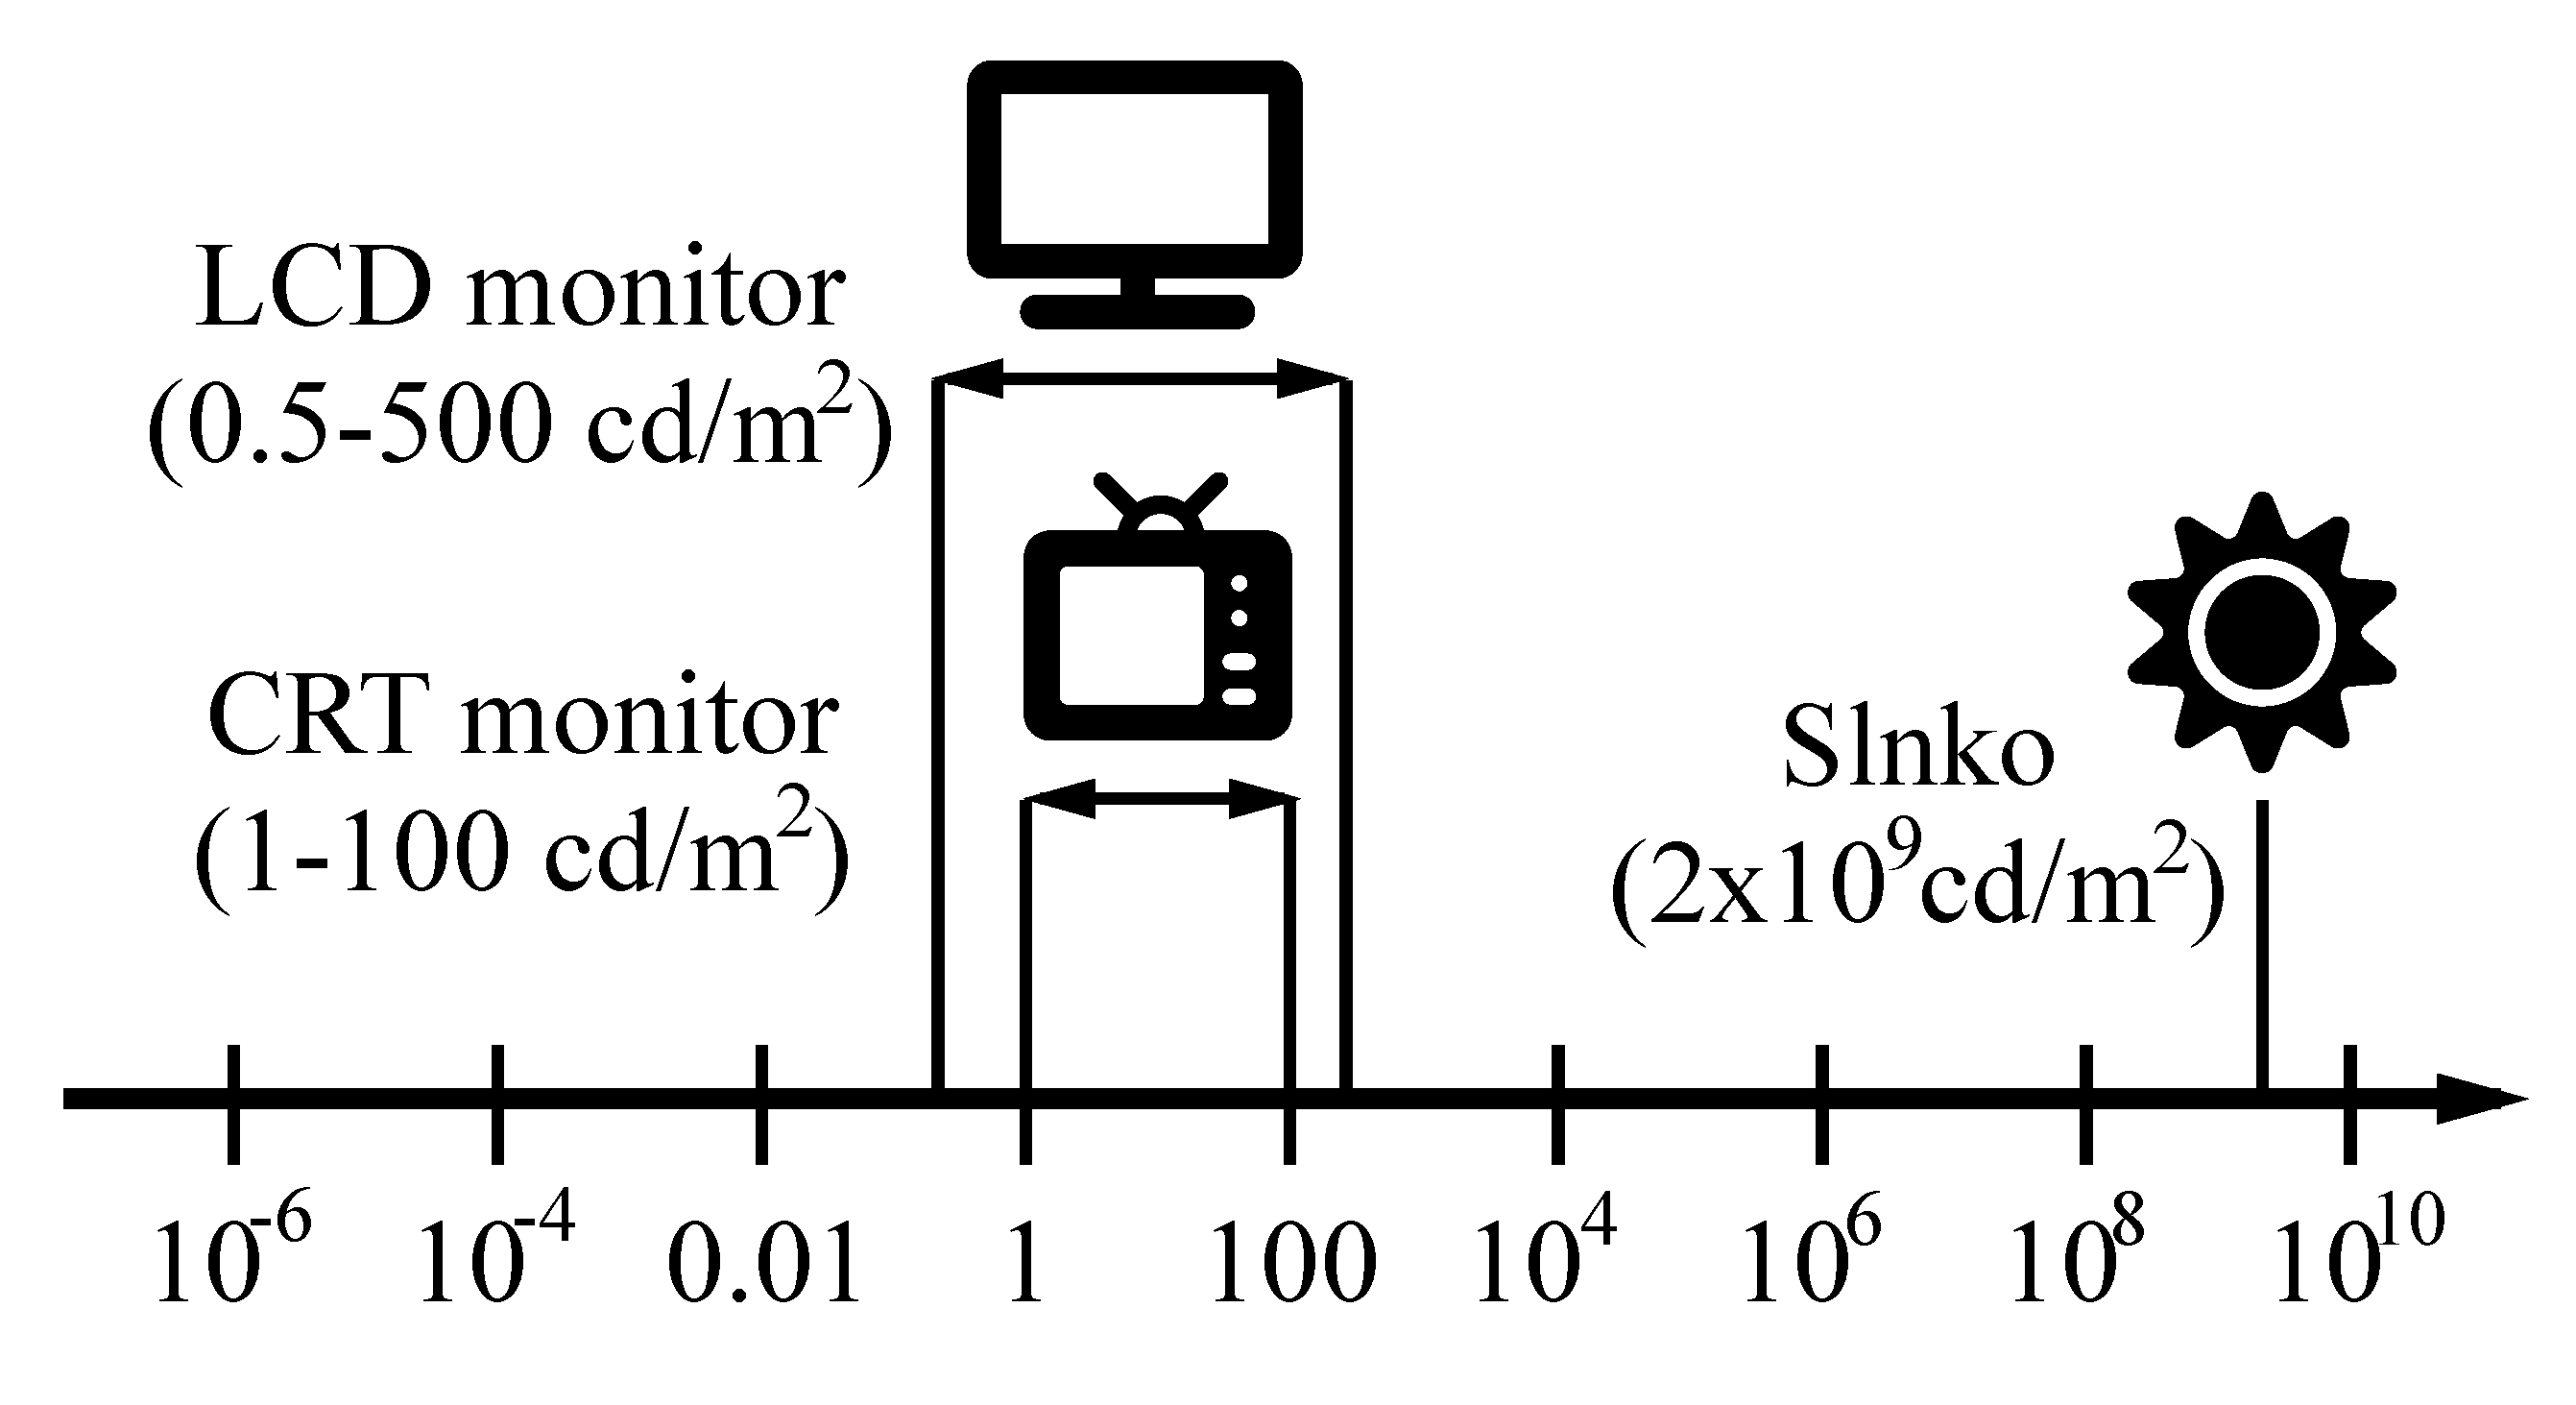
\includegraphics[width=0.6\textwidth]{figures/tonemap/monitor_range}
    \caption{Hodnoty jasu reálneho sveta v porovnaní s rozsahom jasu, 
    ktorý možno zobrazovať na LCD a CRT monitoroch \cite{Mantiuk}}
    \label{fig:luminance_range}
\end{figure}

\subsection*{Mapovanie tónov}

Mapovanie tónov je proces prevodu obrazu s vysokým dynamickým rozsahom na 8-bitový obraz pre farebný kanál, 
s cieľom zachovať čo najväčší počet detailov. Mapovanie tónov znižuje dynamický rozsah alebo kontrastný pomer
celého záberu so zachovaním lokálneho kontrastu. \cite{AHDR}

Existuje viacero metód mapovania tónov a ich ciele môžu byť rozličné v závislosti od konkrétneho využitia.
V niektorých prípadoch je hlavným cieľom vytvárať len esteticky príjemné obrázky, zatiaľ čo iné metódy
reprodukujú čo najväčší počet obrazových detailov alebo maximalizujú kontrast obrazu. Cieľom vykresľovacích 
aplikácií môže byť dosiahnutie čo najväčšej zhody medzi skutočnou scénou a zobrazeným obrázkom, aj keď
zobrazovacie zariadenie nedokáže reprodukovať celý rozsah hodnôt jasu.

\subsection{Operátory mapovania tónov}
\label{sec:Theory-Operators}

Väčšina metód mapovania tónov sa zameriava na susediace pixely a s ich informáciami môže vykonať tónovanie,
napríklad nastavením jasu vo vzťahu k susediacím pixelom. Jedným zo spôsobov je rozostriť oblasť, čo spriemeruje
jas a potom túto informáciu použiť. \cite{ZakladyHDR} Rozostrenie sa neaplikuje na obrázok, iba sa využije
k výpočtom.

V posledných rokoch boli vyvinuté rôzne metódy mapovania tónov, ktoré je môžeme rozdeliť do dvoch základných
typov:
\begin{description}
    \item [Globálne operátory] (priestorovo jednotné) sú nelineárne funkcie založené na svetelných a iných
    globálnych premenných obrazu. Akonáhle je optimálna funkcia odhadnutá podľa konkrétnej snímky, každý pixel
    v obraze je mapovaný rovnakým spôsobom, nezávisle od hodnoty okolitých pixelov v obraze. Tieto techniky 
    sú jednoduché a~rýchle, ale môžu spôsobiť stratu lokálneho kontrastu.
    \cite{AHDR}
    
    \item [Lokálne operátory] (priestorovo sa meniace) sú nelineárnej funkcie, ktorých parametre sa menia
    v každom pixeli podľa vlastností získaných z okolitých oblastí. Inými slovami, efekt metódy sa mení
    pre každý pixel podľa vlastností obrazu na danom mieste. Tieto metódy sú zložitejšie ako globálne
    a môžu vytvárať artefakty, ako napríklad halo efekt alebo kontrastné obrysy a tým môže výstup metódy vyzerať
    nerealisticky. Avšak poskytujú lepší výsledok, pretože ľudské vnímanie je citlivé hlavne na lokálny kontrast.
    \cite{AHDR}
\end{description}

Medzi najznámejšie metódy mapovania tónov patria:
\begin{description}
    \item [Bilaterálny filter]
    (Durand a Dorsey 2002) - lokálny operátor, ktorý zachováva detaily. Metóda sa pokúša zobraziť obrazy HDR
    rozložením obrazu na základnú vrstvu a~vrstvu detailov. V základnej vrstve je kontrast skomprimovaný
    bilaterálnym filtrom, ktorý chráni hrany. \cite{TMODurand}

    \item [Fotografická reprodukcia]
    (Reinhard a spol. 2002) - tento operátor simuluje techniku "dodging and burning", ktorá bola používaná
    v počiatkoch fotografie a dovoľuje vytvárať rozličné expozície naprieč fotografiou. Lokálny operátor
    obsahuje aj jednoduchšiu globálnu verziu. \cite{TMOReinhard}
    
    \item [Logaritmické mapovanie]
    (Drago a spol. 2003) - metóda redukuje pomer kontrastu logaritmickou kompresiou hodnôt jasu,
    napodobňujúc ľudské vnímanie svetla. Zachováva detaily a kontrast scény. \cite{TMODrago}

    \item [Perceptuálny rámec pre kontrastné spracovanie HDR]
    (Mantiuk a spol.) - metóda vytvára rámec pre spracovanie obrazu v priestore vizuálnej odozvy, v ktorej
    kontrastné hodnoty priamo korelujú so svojou viditeľnosťou v obraze. Rámec zahŕňa transformáciu obrazu
    z jasového priestoru na pyramídu obrázkov s nízkym kontrastom a potom do priestoru vizuálnej
    odozvy. \cite{TMOMantiuk}

    \item [Kompresia gradiendom]
    (Fattal a spol.) - metóda znižuje rozsah gradiendového poľa jasu. Obraz s nízkym dynamickým rozsahom
    je získaný riešením Poissonovej rovnice na modifikovanom gradiendovom poli. Metóda je schopná dobrej
    kompresie dynamického rozsahu, pričom zachováva jemné detaily a vyhýba sa bežným artefaktom. \cite{TMOFattal}

    \item [Úprava histogramu] (Larson a spol. 1997) - cieľom operátora je vytvárať HDR fotografie, ktoré
    zachovávajú realistickosť scény. Obsahuje modely citlivosti človeka na kontrast, farby, ostrosť zraku
    a osvetlenie, podľa ktorých sa vytvárajú obrazy zodpovedajúce skúsenostiam diváka na skutočnej scéne.
    \cite{AHDR}

    \item [Model iCAM]
    (Johnson a Fairchild 2003) - model vzhľadu obrazu, ktorý bol rozšírený pre zobrazovanie HDR obrázkov
    na displej. iCAM sa pokúša určiť perceptuálnu odozvu voči priestorovo zložitým podnetom a dokáže predvídať
    vzhľad HDR obrazu. \cite{TMOFairchild}
    
    \item [Lokálny model prispôsobenia očí]
    (Ledda a spol. 2004) - simuluje reakciu sietnice na~jas, avšak v tomto prípade je proces úplne lokalizovaný,
    čo umožňuje dobrú kompresiu dynamického rozsahu. Tento model je podobný modelu Pattanaika a spol. z roku 2000.
    \cite{TMOLedda}
\end{description}
